



\section{Paradigma No 04 – Programación Funcional} 

\begin{enumerate}[1.]
	\item Programacion funcional:
\\
La Programación Funcional  es una forma en la cual podemos resolver diferentes problemáticas ya que estaremos trabajando principalmente con funciones, evitaremos los datos mutables, así como el hecho de compartir estados entre funciones.
\\	
\begin{center}
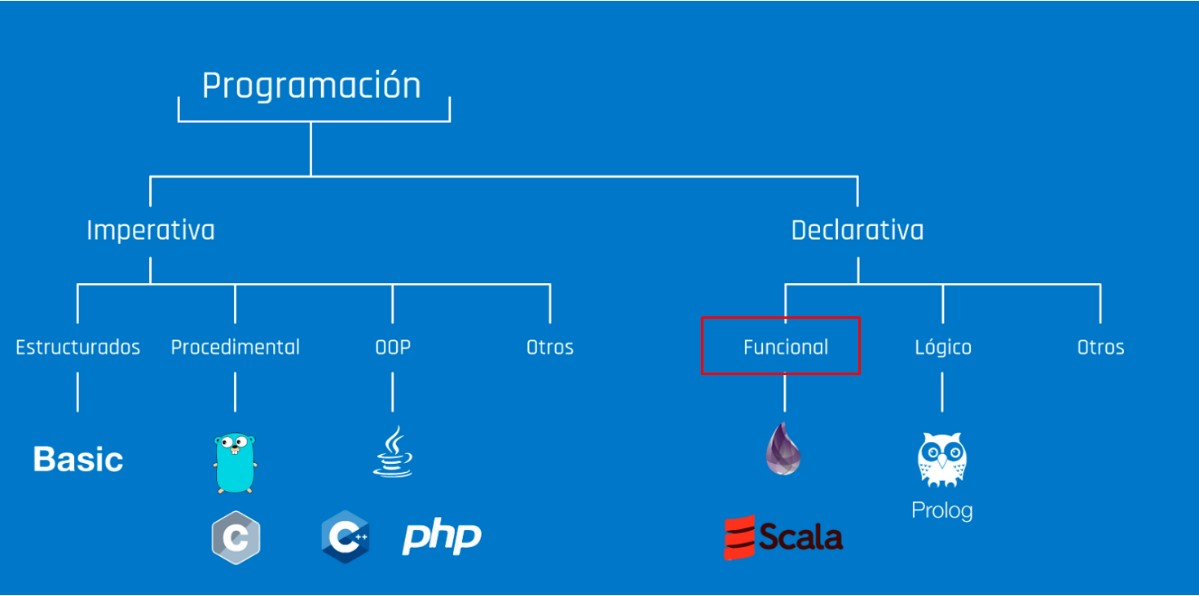
\includegraphics[scale=0.80]{./Imagenes/img04.jpg} 
\end{center}
Las funciones serán tratadas como ciudadanos de primera clase. Las funciones podrán ser asignadas a variables además podrán ser utilizadas como entrada y salida de otras funciones
\\
\\	
Ejemplo
\\
De forma tradicional imperativa tendríamos que especificar como lo haremos
\begin{center}
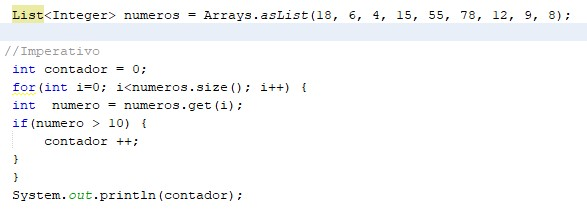
\includegraphics[scale=0.55]{./Imagenes/img05.jpg} 
\end{center}


Pero de forma declarativa o programación funcional tendríamos
\begin{center}
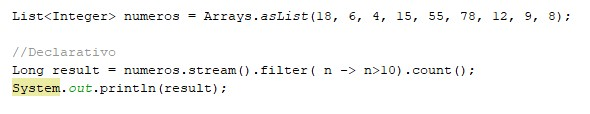
\includegraphics[scale=0.55]{./Imagenes/img06.jpg} 
\end{center}




\end{enumerate}






 